\newcommand{\stickman}[2]{
    \node[circle,fill,minimum size=2.5mm,#2] (head) at #1 {};
    \node[rounded corners=1pt,minimum height=0.65cm,minimum width=0.2cm,fill,below = 0.5pt of head,#2] (body) {};
    \draw[line width=0.5mm,round cap-round cap,#2] ([shift={(1pt,-0.5pt)}]body.north east) --++(-90:3mm);
    \draw[line width=0.5mm,round cap-round cap,#2] ([shift={(-1pt,-0.5pt)}]body.north west)--++(-90:3mm);
    \draw[thick,white,-round cap] (body.south) --++(90:2.75mm);
}

\newsavebox{\heterogeneity}
\sbox{\heterogeneity}{
    \begin{tikzpicture}
        \node [
            single arrow,
            top color=red,
            bottom color=red!30!blue,
            %single arrow head extend=3pt,
            transform shape,
            minimum height=0.5cm,
            text width=3cm,rotate=90
        ] (out) at (1.6, -1.8){};

        \node [
            single arrow,
            right color=red,
            left color=red!30!blue,
            %single arrow head extend=3pt,
            transform shape,
            minimum height=0.5cm,
            text width=4cm,
        ] (out) at (3.6, -3.5){};

        \stickman{(2.1, -0.8)}{red}
        \stickman{(3.5, -1.7)}{red!50!blue}
        \stickman{(2.2, -2.3)}{red!95!blue}
        \stickman{(3.8, -1.2)}{red}
        \stickman{(4.7, -2.1)}{red!60!blue}
        \stickman{(5.2, -1.1)}{red!72!blue}
        \stickman{(4.2, -0.5)}{red!70!blue}

        \stickman{(2.6, -2)}{red!93!blue}
        \stickman{(4.0, -2.4)}{red!88!blue}
        \stickman{(2.8, -0.9)}{red!71!blue}
        \stickman{(4.6, -1)}{red!82!blue}
        \stickman{(5.1, -2.0)}{red!86!blue}
        \stickman{(3.3, -2.3)}{red!97!blue}
        \stickman{(3.3, -0.5)}{red!65!blue}
    \end{tikzpicture}
}

\begin{frame}{Background: Predictive clinical neuroscience}
    \begin{tikzpicture}
        \node[] at (-5.25, 3.5) {};
        \node[] at (5.25, -3.5) {};

        \visible<1,3>{
            \node[inner sep=0pt] (input) at (-3.35, 1.5) {
                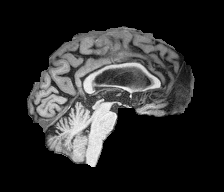
\includegraphics[height=2cm]{data/mri_sagittal.png}
            };

            \node[draw=black, minimum height=2cm, minimum width=3cm, align=center, font=\normalfont\linespread{0.95}\selectfont] (model) at (0.3, 1.5) {
                Predictive\\model
            };
            \node[align=left, inner sep=0pt,font=\normalfont\linespread{0.95}\selectfont] (output) at (3.7, 1.5) {
                Clinically\\relevant\\predictions
            };

            \draw[-stealth, line width=3pt, gray] (input) -- (model);
            \draw[-stealth, line width=3pt, gray] (model) -- (output);
        }

        \visible<2>{
            \node[
                font=\fontsize{10}{10}\selectfont\bfseries,
                align=center,
                anchor=west
            ] at (-4.5, -1.75) {
                Structural Magnetic\\
                Resonance Imaging (MRI) scans
            };

            \node[label=below:\small{Side}] (side) at (-3.25, 1.5) {
                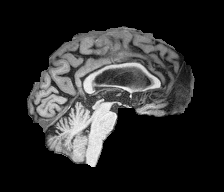
\includegraphics[height=2cm]{data/mri_sagittal.png}
            };

            \node[label=below:\small{Above}] at (0, 1.5) {
                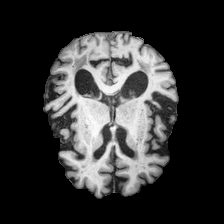
\includegraphics[height=2cm]{data/mri_axial.png}
            };

            \node[label=below:\small{Front}] at (3.25, 1.5) {
                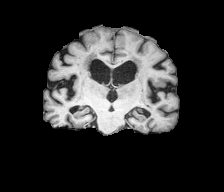
\includegraphics[height=2cm]{data/mri_coronal.png}
            };

            \node[anchor=east] (threed) at (4.5, -1.75) {
                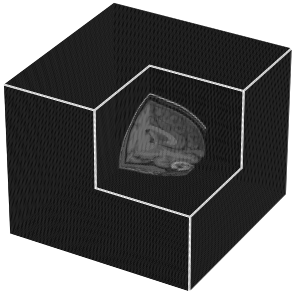
\includegraphics[height=3cm]{data/3d_bert.png}
            };
        }
        \visible<4>{
            \node [
                double arrow,
                draw=black,
                right color=white,
                left color=black,
                %single arrow head extend=3pt,
                transform shape,
                minimum height=2cm,
                text width=9cm,
            ] (out) at (0, -1.25){};

            \node[align=center, font=\normalfont\linespread{0.8}\selectfont] at (-3, -0.5) {
                Parkinson's\\disease
            };
            \node[align=center, font=\normalfont\linespread{0.8}\selectfont] at (-3.5, 0.4) {
                Multiple\\sclerosis
            };
            \node[align=center, font=\normalfont\linespread{0.8}\selectfont] at (-1.5, 0.3) {
                Dementia
            };
            \node[align=center, font=\normalfont\linespread{0.8}\selectfont] at (3, -0.7) {
                Schizophrenia
            };
            \node[align=center, font=\normalfont\linespread{0.8}\selectfont] at (4.2, 0) {
                Bipolar\\disorder
            };
            \node[align=center, font=\normalfont\linespread{0.8}\selectfont] at (2.4, 0.1) {
                Depression
            };
        }
        \visible<5>{
            \node[] at (0, 0) {
                \usebox{\heterogeneity}
            };
        }
        \visible<6,9>{
            \draw[dashed] (-1.2, 1.1) -- (1.2, -2.2);
        }
        \visible<6>{
            \stickman{(0.4, 0)}{red!80!blue}
            \stickman{(0.9, -0.5)}{red!95!blue}
            \stickman{(0, 0.7)}{red!92!blue}
            \stickman{(1.4, 0.2)}{red}
            \stickman{(1.0, 0.9)}{red!75!blue}

            \stickman{(-0.1, -1)}{blue!80!red}
            \stickman{(-0.7, -0.8)}{blue!85!red}
            \stickman{(-0.6, 0.3)}{blue!75!red}
            \stickman{(0.5, -1.4)}{blue!95!red}
            \stickman{(-1.1, -0.1)}{blue}

            \node[font=\scriptsize\selectfont] at (-0.1, 1.3) {
                Patients
            };
            \node[font=\scriptsize\selectfont] at (-0.8, -2.1) {
                Controls
            };
        }
        \visible<7-9>{
            \stickman{(0.4, 0)}{red!80!blue}
            \stickman{(0.9, -0.5)}{red!95!blue}
            \stickman{(0, 0.7)}{red!92!blue}
            \stickman{(1.4, 0.2)}{red}
            \stickman{(1.0, 0.9)}{red!75!blue}

            \stickman{(-0.1, -1)}{red!80!blue}
            \stickman{(-0.7, -0.8)}{red!85!blue}
            \stickman{(-0.6, 0.3)}{red!75!blue}
            \stickman{(0.5, -1.4)}{red!95!blue}
            \stickman{(-1.1, -0.1)}{red}
        }
        \visible<7>{
            \node [
                single arrow,
                fill=red,
                transform shape,
                minimum height=3cm,
                text width=2.5cm,
                minimum width=1cm
            ] (out) at (3.2, 0) {};
            \node[text=white] at (3.2, 0) {
                \footnotesize{Prognosis}
            };
        }
        \visible<8>{
            \draw[-stealth] (-0.61, 1.18) -- (-0.61, 0.48);
            \draw[-stealth] (1, 1.7) -- (1, 1.08);
            \draw[-stealth] (0.9, -2.07) -- (0.9, -1.37);
        }
        \visible<9>{
            \node[font=\scriptsize\selectfont] at (-0.1, 1.3) {
                Subtype 1
            };
            \node[font=\scriptsize\selectfont] at (-0.8, -2.1) {
                Subtype 2
            };
        }
    \end{tikzpicture}
\end{frame}

\newcommand{\nnneuron}[3]{
    \node[circle, minimum size=0.3cm, inner sep=0pt, draw=none, fill=#3, draw=#3] (#2) at #1 {};
}
\newcommand{\neuronconnection}[4]{
    \begin{scope}[transparency group, opacity=0.5]
        \draw[#4,line width=1.5pt, #3] (#1) to [in=180, out=0] (#2);
    \end{scope}
}
\newcommand{\lrpconnection}[4]{
    \begin{scope}[transparency group, opacity=0.5]
        \draw[#4,line width=1.5pt, #3] (#1) to [in=0, out=180] (#2);
    \end{scope}
}

\newcommand{\artificialneuron}[5]{
    \node[
        circle,
        fill=#5,
        draw=none,
        minimum size=13pt,
        font=\tiny\selectfont,
        text depth=0,
        inner sep=0pt,
        text=white!90
    ] (#4) at (#1, #2) {#3};
}
\newcommand{\connection}[4]{
    \draw[-stealth, line width=1pt,#3] #1 -- #2 #4;
}

\newcommand{\mathplot}[1]{
    \begin{tikzpicture}
        \node[] at (-4, -1.5) {};
        \node[] at (4, 1.5) {};

        \ifnum#1=0
            \artificialneuron{-0.5}{1}{$n_{00}$}{n00}{black!65}
            \artificialneuron{-0.5}{0.5}{$n_{01}$}{n01}{black!55}
            \artificialneuron{-0.5}{0}{$n_{02}$}{n02}{black!98}

            \artificialneuron{0.5}{0.5}{$n_{10}$}{n10}{black!82}

            \connection{(n00)}{(n10)}{black!45}{node [midway, above, font=\tiny\selectfont, text=black, yshift=-0.05cm] {$w_0$}}
            \connection{(n01)}{(n10)}{black!92}{node [above, font=\tiny\selectfont, text=black, pos=0.35, yshift=-0.11cm] {$w_1$}}
            \connection{(n02)}{(n10)}{black!78}{node [midway, below, font=\tiny\selectfont, text=black, yshift=0.03cm] {$w_2$}}

            \connection{($ (n00.west) - (0.5, 0) $)}{(n00)}{black!65}{}
            \connection{($ (n01.west) - (0.5, 0) $)}{(n01)}{black!55}{}
            \connection{($ (n02.west) - (0.5, 0) $)}{(n02)}{black!98}{}

            \connection{(n10)}{($ (n10.east) + (0.5, 0) $)}{black!82}{}

            \node[anchor=west, font=\tiny\selectfont] at ($ (n10.east) + (0.5, 0) $) {$\hat{y}$};

            \node[anchor=east, font=\tiny\selectfont] at ($ (n00.west) - (0.5, 0) $) {$x_0$};
            \node[anchor=east, font=\tiny\selectfont] at ($ (n01.west) - (0.5, 0) $) {$x_1$};
            \node[anchor=east, font=\tiny\selectfont] at ($ (n02.west) - (0.5, 0) $) {$x_2$};

            \node[font=\footnotesize\selectfont, anchor=north] at (0, -0.25) {
                $\hat{y}=f\left({\color{red}\sum\limits_i^N w_i \cdot n_{0i}}\right)$
            };
        \fi

        \ifnum#1=1
            \artificialneuron{-0.5}{1}{$n_{00}$}{n00}{red!95!black}
            \artificialneuron{-0.5}{0.5}{$n_{01}$}{n01}{red!80!black}
            \artificialneuron{-0.5}{0}{$n_{02}$}{n02}{blue!50!black}

            \artificialneuron{0.5}{0.5}{$n_{10}$}{n10}{red}

            \connection{(n10)}{(n00)}{red!95!black}{}
            \connection{(n10)}{(n01)}{red!80!black}{}
            \connection{(n10)}{(n02)}{blue!50!black}{}

            \connection{(n00)}{($ (n00.west) - (0.5, 0) $)}{red!95!black}{}
            \connection{(n01)}{($ (n01.west) - (0.5, 0) $)}{red!80!black}{}
            \connection{(n02)}{($ (n02.west) - (0.5, 0) $)}{blue!50!black}{}

            \connection{($ (n10.east) + (0.5, 0) $)}{(n10)}{red}{}

            \node[anchor=west, font=\tiny\selectfont] at ($ (n10.east) + (0.5, 0) $) {$R_{10}$};

            \node[anchor=east, font=\tiny\selectfont] at ($ (n00.west) - (0.5, 0) $) {$R_{00}$};
            \node[anchor=east, font=\tiny\selectfont] at ($ (n01.west) - (0.5, 0) $) {$R_{01}$};
            \node[anchor=east, font=\tiny\selectfont] at ($ (n02.west) - (0.5, 0) $) {$R_{02}$};

            \node[font=\footnotesize\selectfont, anchor=north] at (0, -0.25) {
                $R_{0i} = \sum\limits_j \dfrac{n_{0i}w_i}{\sum\limits_k n_{0k}w_k}R_{1j}$
            };
        \fi

    \end{tikzpicture}
}

\newsavebox{\mathforward}
\sbox{\mathforward}{
    \mathplot{0}
}

\newsavebox{\mathbackward}
\sbox{\mathbackward}{
    \mathplot{1}
}

\begin{frame}{Background: Explainable artificial intelligence}
    \begin{tikzpicture}
        \node[] at (-5.25, 3.5) {};
        \node[] at (5.25, -3.5) {};

        \visible<1>{
            \node[draw=black, minimum height=2cm, minimum width=3cm, align=center, font=\normalfont\linespread{0.95}\selectfont] (model) at (0.3, 1.5) {
                Predictive\\model
            };
        }

        \visible<1-2>{
            \node[inner sep=0pt] (input) at (-3.35, 1.5) {
                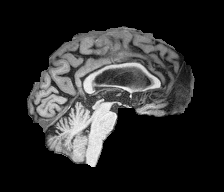
\includegraphics[height=2cm]{data/mri_sagittal.png}
            };

            \node[align=left, inner sep=0pt,font=\normalfont\linespread{0.95}\selectfont] (output) at (3.7, 1.5) {
                Clinically\\relevant\\predictions
            };

            \draw[-stealth, line width=3pt, gray] (input) -- (model);
            \draw[-stealth, line width=3pt, gray] (model) -- (output);
        }
        \visible<2-8>{
            \node[draw=black, minimum height=2cm, minimum width=3cm, align=center, font=\normalfont\linespread{0.95}\selectfont, label=above:\footnotesize{Artificial neural network}] (model) at (0.3, 1.5) {};
        }
        \visible<2-3>{
            \nnneuron{(-0.8, 2.2)}{n00}{gray}
            \nnneuron{(-0.8, 1.85)}{n01}{gray}
            \nnneuron{(-0.8, 1.5)}{n02}{gray}
            \nnneuron{(-0.8, 1.15)}{n03}{gray}
            \nnneuron{(-0.8, 0.8)}{n04}{gray}
            \nnneuron{(0.3, 1.85)}{n10}{gray}
            \nnneuron{(0.3, 1.5)}{n11}{gray}
            \nnneuron{(0.3, 1.15)}{n12}{gray}
            \nnneuron{(1.4, 1.5)}{n20}{gray}

            \neuronconnection{n00}{n10}{gray}{-}
            \neuronconnection{n00}{n11}{gray}{-}
            \neuronconnection{n00}{n12}{gray}{-}
            \neuronconnection{n01}{n10}{gray}{-}
            \neuronconnection{n01}{n11}{gray}{-}
            \neuronconnection{n01}{n12}{gray}{-}
            \neuronconnection{n02}{n10}{gray}{-}
            \neuronconnection{n02}{n11}{gray}{-}
            \neuronconnection{n02}{n12}{gray}{-}
            \neuronconnection{n03}{n10}{gray}{-}
            \neuronconnection{n03}{n11}{gray}{-}
            \neuronconnection{n03}{n12}{gray}{-}
            \neuronconnection{n04}{n10}{gray}{-}
            \neuronconnection{n04}{n11}{gray}{-}
            \neuronconnection{n04}{n12}{gray}{-}

            \neuronconnection{n10}{n20}{gray}{-}
            \neuronconnection{n11}{n20}{gray}{-}
            \neuronconnection{n12}{n20}{gray}{-}
        }
        \visible<3>{
            \node[anchor=east, text depth=0] (x0) at (-1.8, 2) {
                Temperature
            };
            \node[anchor=east, text depth=0] (x1) at (-1.8, 1.5) {
                CRP
            };
            \node[anchor=east, text depth=0] (x2) at (-1.8, 1) {
                Age
            };

            \neuronconnection{x0}{n00}{gray}{-stealth}
            \neuronconnection{x0}{n01}{gray}{-stealth}
            \neuronconnection{x0}{n02}{gray}{-stealth}
            \neuronconnection{x0}{n03}{gray}{-stealth}
            \neuronconnection{x0}{n04}{gray}{-stealth}
            \neuronconnection{x1}{n00}{gray}{-stealth}
            \neuronconnection{x1}{n01}{gray}{-stealth}
            \neuronconnection{x1}{n02}{gray}{-stealth}
            \neuronconnection{x1}{n03}{gray}{-stealth}
            \neuronconnection{x1}{n04}{gray}{-stealth}
            \neuronconnection{x2}{n00}{gray}{-stealth}
            \neuronconnection{x2}{n01}{gray}{-stealth}
            \neuronconnection{x2}{n02}{gray}{-stealth}
            \neuronconnection{x2}{n03}{gray}{-stealth}
            \neuronconnection{x2}{n04}{gray}{-stealth}

            \node[anchor=west, text depth=0] (y) at (2.4, 1.5) {
                Flu?
            };

            \neuronconnection{n20}{y}{gray}{-stealth}
        }

        \visible<4-8>{
            \node[anchor=west, text depth=0] (y) at (2.4, 1.5) {
                1 (Yes)
            };
        }
        \visible<4-6>{
            \nnneuron{(-0.8, 2.2)}{n00}{black!80}
            \nnneuron{(-0.8, 1.85)}{n01}{black!60}
            \nnneuron{(-0.8, 1.5)}{n02}{black!95}
            \nnneuron{(-0.8, 1.15)}{n03}{black!20}
            \nnneuron{(-0.8, 0.8)}{n04}{black!45}
            \nnneuron{(0.3, 1.85)}{n10}{black!52}
            \nnneuron{(0.3, 1.5)}{n11}{black!83}
            \nnneuron{(0.3, 1.15)}{n12}{black}
            \nnneuron{(1.4, 1.5)}{n20}{black!75}

            \neuronconnection{n00}{n10}{black!70}{-}
            \neuronconnection{n00}{n11}{black!32}{-}
            \neuronconnection{n00}{n12}{black!50}{-}
            \neuronconnection{n01}{n10}{black!65}{-}
            \neuronconnection{n01}{n11}{black!92}{-}
            \neuronconnection{n01}{n12}{black!50}{-}
            \neuronconnection{n02}{n10}{black!25}{-}
            \neuronconnection{n02}{n11}{black!67}{-}
            \neuronconnection{n02}{n12}{black!73}{-}
            \neuronconnection{n03}{n10}{black!42}{-}
            \neuronconnection{n03}{n11}{black!18}{-}
            \neuronconnection{n03}{n12}{black!23}{-}
            \neuronconnection{n04}{n10}{black!40}{-}
            \neuronconnection{n04}{n11}{black!62}{-}
            \neuronconnection{n04}{n12}{black!52}{-}

            \neuronconnection{n10}{n20}{black!52}{-}
            \neuronconnection{n11}{n20}{black!83}{-}
            \neuronconnection{n12}{n20}{black!70}{-}

            \node[anchor=east, text depth=0] (x0) at (-1.8, 2) {
                38.5
            };
            \node[anchor=east, text depth=0] (x1) at (-1.8, 1.5) {
                50
            };
            \node[anchor=east, text depth=0] (x2) at (-1.8, 1) {
                35
            };

            \neuronconnection{x0}{n00}{gray}{-stealth}
            \neuronconnection{x0}{n01}{gray}{-stealth}
            \neuronconnection{x0}{n02}{gray}{-stealth}
            \neuronconnection{x0}{n03}{gray}{-stealth}
            \neuronconnection{x0}{n04}{gray}{-stealth}
            \neuronconnection{x1}{n00}{gray}{-stealth}
            \neuronconnection{x1}{n01}{gray}{-stealth}
            \neuronconnection{x1}{n02}{gray}{-stealth}
            \neuronconnection{x1}{n03}{gray}{-stealth}
            \neuronconnection{x1}{n04}{gray}{-stealth}
            \neuronconnection{x2}{n00}{gray}{-stealth}
            \neuronconnection{x2}{n01}{gray}{-stealth}
            \neuronconnection{x2}{n02}{gray}{-stealth}
            \neuronconnection{x2}{n03}{gray}{-stealth}
            \neuronconnection{x2}{n04}{gray}{-stealth}

            \neuronconnection{n20}{y}{black}{-stealth}
        }
        \visible<5,9>{
            \node[] at (0, -1.5) {
                \usebox{\mathforward}
            };
        }
        \visible<6-8,10>{
            \node[] at (0, -1.5) {
                \usebox{\mathbackward}
            };
        }
        \visible<7-8>{
            \nnneuron{(-0.8, 2.2)}{n00}{red!75!black}
            \nnneuron{(-0.8, 1.85)}{n01}{red!90!black}
            \nnneuron{(-0.8, 1.5)}{n02}{blue!10!black}
            \nnneuron{(-0.8, 1.15)}{n03}{blue!40!black}
            \nnneuron{(-0.8, 0.8)}{n04}{red!45!black}
            \nnneuron{(0.3, 1.85)}{n10}{red!90!black}
            \nnneuron{(0.3, 1.5)}{n11}{red!50!black}
            \nnneuron{(0.3, 1.15)}{n12}{blue!10!black}
            \nnneuron{(1.4, 1.5)}{n20}{red!95!black}

            \node[anchor=east, text depth=0, text=red] (x0) at (-1.8, 2) {
                0.5
            };
            \node[anchor=east, text depth=0, text=red] (x1) at (-1.8, 1.5) {
                0.7
            };
            \node[anchor=east, text depth=0, text=blue] (x2) at (-1.8, 1) {
                -0.2
            };

            \lrpconnection{y}{n20}{red!95}{-stealth}

            \lrpconnection{n20}{n10}{red!90!black}{-}
            \lrpconnection{n20}{n11}{red!50!black}{-}
            \lrpconnection{n20}{n12}{blue!10!black}{-}

            \lrpconnection{n10}{n00}{red!10!black}{-}
            \lrpconnection{n10}{n01}{red!70!black}{-}
            \lrpconnection{n10}{n02}{blue!10!black}{-}
            \lrpconnection{n10}{n03}{blue!50!black}{-}
            \lrpconnection{n10}{n04}{red!90!black}{-}

            \lrpconnection{n11}{n00}{red!60!black}{-}
            \lrpconnection{n11}{n01}{blue!70!black}{-}
            \lrpconnection{n11}{n02}{red!20!black}{-}
            \lrpconnection{n11}{n03}{blue!20!black}{-}
            \lrpconnection{n11}{n04}{red!40!black}{-}

            \lrpconnection{n12}{n00}{red!80!black}{-}
            \lrpconnection{n12}{n01}{blue!20!black}{-}
            \lrpconnection{n12}{n02}{blue!40!black}{-}
            \lrpconnection{n12}{n03}{red!40!black}{-}
            \lrpconnection{n12}{n04}{red!70!black}{-}


            \lrpconnection{n00}{x0}{red!40!black}{-stealth}
            \lrpconnection{n00}{x1}{red!70!black}{-stealth}
            \lrpconnection{n00}{x2}{red!20!black}{-stealth}

            \lrpconnection{n01}{x0}{red!80!black}{-stealth}
            \lrpconnection{n01}{x1}{red!20!black}{-stealth}
            \lrpconnection{n01}{x2}{blue!20!black}{-stealth}

            \lrpconnection{n02}{x0}{red!50!black}{-stealth}
            \lrpconnection{n02}{x1}{blue!10!black}{-stealth}
            \lrpconnection{n02}{x2}{blue!70!black}{-stealth}

            \lrpconnection{n03}{x0}{blue!20!black}{-stealth}
            \lrpconnection{n03}{x1}{blue!60!black}{-stealth}
            \lrpconnection{n03}{x2}{blue!40!black}{-stealth}

            \lrpconnection{n04}{x0}{red!90!black}{-stealth}
            \lrpconnection{n04}{x1}{blue!10!black}{-stealth}
            \lrpconnection{n04}{x2}{red!20!black}{-stealth}

        }
        \visible<8>{
            \draw[] (-2.7, 0.75) -- (-1.7, 0.75);
            \node[anchor=east, text depth=0] (x2) at (-1.8, 0.5) {
                =1.0
            };
        }
        \visible<9>{
            \node[] at (0.4, 1.7) {
                \usebox{\cnnpatient}
            };
        }
        \visible<10>{
            \node[] at (0.4, 1.7) {
                \usebox{\lrppatient}
            };
        }
        \visible<11>{
            \node[] (side) at (-3.25, 0) {
                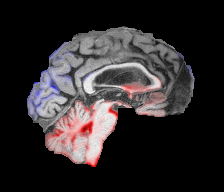
\includegraphics[height=2.5cm]{data/combined_sagittal.png}
            };

            \node[] at (0, 0) {
                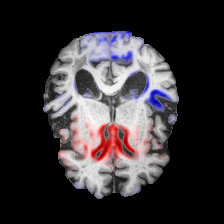
\includegraphics[height=2.5cm]{data/combined_axial.png}
            };

            \node[] at (3.25, 0) {
                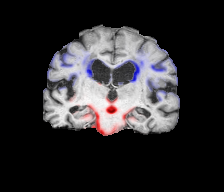
\includegraphics[height=2.5cm]{data/combined_coronal.png}
            };
        }
    \end{tikzpicture}
\end{frame}
